\documentclass[a4paper,12pt,oneside]{article}

\usepackage{graphicx}  % for including images
\usepackage[a4paper,top=4.2cm,bottom=4.2cm,left=3.5cm,right=3.5cm]{geometry} % for setting page size and margins


\begin{document}
	
	\begin{titlepage}
		\begin{center}
			\vspace*{1cm}
			
			\Huge
			\textbf{BookIT}
			
			\vspace{0.5cm}
			\LARGE
			Virtual Library Documentation
	
			
			\vfill
			\vspace{0.8cm}
			
			\Large
			UMCS 2022
			
		\end{center}
	\end{titlepage}
	
	\section{Project setup}
	
	Project is a ASP.NET, MVC based web application. Things needed to set this project up are:
	
	\begin{itemize}
		\item Visual Studio 2022
		\item MSSQL Server
		\item SSMS (not necessarily needed but it's perfect to manage database)
	\end{itemize}

	\subsection{Open project in VS 2022}
	If things listed above are installed you can open project in Visual Studio 2022 or find "bkit.sln" file and it will automaticly open editor.
	
	\begin{figure}[h]
		\centering
		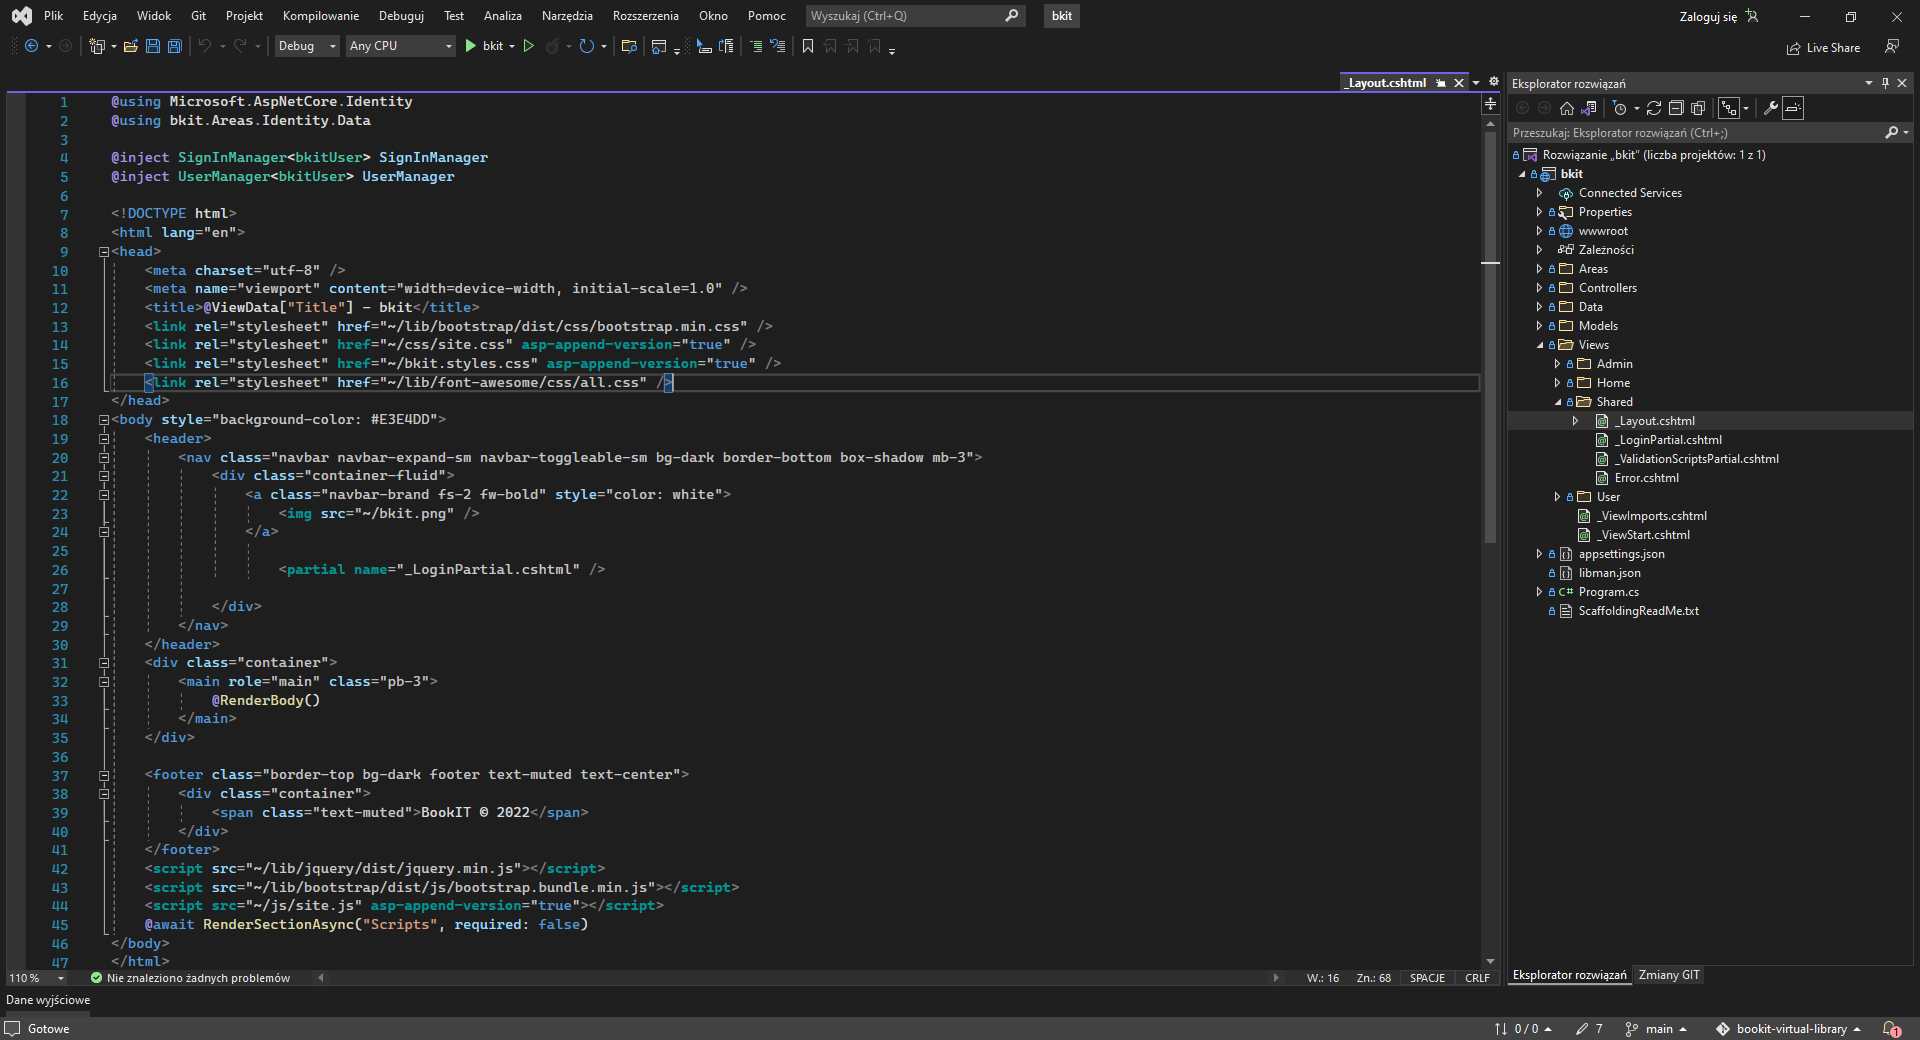
\includegraphics[width=1\textwidth]{img/vsstudio}
		\caption{Visual Studio 2022}
	\end{figure}

	\newpage
	
	\subsection{Import database}
	To import database first open SSMS and make sure SQL Server runs on your computer. After successfull login right click on "Databases" folder and then click "Import Datatier Application" and import "bookit.bacpac" file located in "db" folder.
	
	\begin{figure}[h]
		\centering
		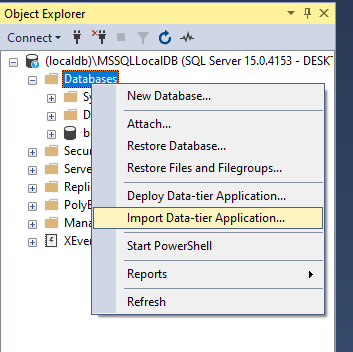
\includegraphics[width=1\textwidth]{img/import}
		\caption{Importing database}
	\end{figure}

	\setlength{\parindent}{0pt}After thet you should be able to start project in VS 2022 by pressing play button.
	\newpage
	
	\section{About project}
	The project is a ASP.NET MVC based application. Project has four basic functionalities CRUD:
	\begin{itemize}
		\item  CREATE
		\item  READ
		\item  UPDATE
		\item  DELETE
	\end{itemize}
	The project is a simple virtual library system.
	
	\subsection{Functionalities}
	
	\subsubsection{Users and roles}
	System has a role based login system. You can log into one of two types of account:
	
	\begin{itemize}
		\item  Admin 
		\item  User
	\end{itemize}


	\setlength{\parindent}{0pt}New users can register using register form.
	
	\subsubsection{CRUD}
	System has implemented CRUD functionalities. CREATE, UPDATE and DELETE options are only given for admin users as well as READ option (listing books from database). Normal user can see books stored in database, borrow and return them.
	
	\newpage
	
	\section{Models, Views, Controllers}
	BookIT system uses 3 data models, views divided based on user (admin user, normal user, anonymus user) and 3 controllers.
	
	\begin{figure}[h]
		\centering
		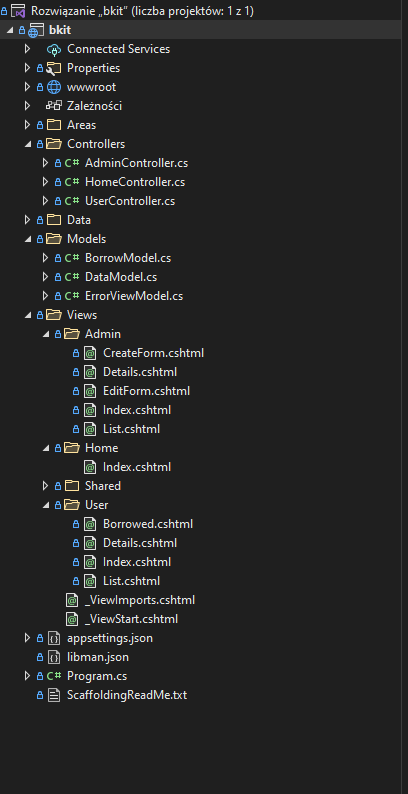
\includegraphics[width=0.57\textwidth]{img/mvc}
		\caption{MVC}
	\end{figure}

	\newpage
	
	\subsection{Models}
	\begin{itemize}
		\item  BorrowModel (Borrowings) 
		\item  DataModel (Books)
		\item  ErrorViewModel (Errors)
	\end{itemize}

	\subsection{Views}
	\begin{itemize}
		\item  Admin Views (Admin subpages) 
		\item  Home View (Landing page)
		\item  User Views (User subpages)
	\end{itemize}

	\subsection{Controllers}
	\begin{itemize}
		\item  AdminController (Admin functionalities) 
		\item  HomeController (Home page functionalities)
		\item  UserControllers (User functionalities)
	\end{itemize}
	
	\section{Information from creator}
	Project was developed for .NET labs. It was my first contact with .NET. If something doesn't work for you that's a shame, because it works perfectly fine for me xD.
	
\end{document}
